
\begin{enumerate}
\item 
\question{If I want a circuit to block DC current but allow AC current, should I use an inductor or a capacitor?}
\solution{Capacitor}
\explanation{Capacitors allow AC current but block DC current.}
\item 
\question{If I want a circuit to allow DC current but block AC current, should I use an inductor or a capacitor?}
\solution{Inductor}
\explanation{Inductors allow DC current but block AC current.}
\item 
\question{Why are inductors used so much in systems that interact with the outside world?}
\solution{Inductors create a magnetic field which can be used to move other components.}
\item 
\question{Why does inductive kick happen?}
\solution{In an inductor, the magnetic field is maintained through current flow through the inductor.  If the current decreases, the magnetic field cannot be maintained, and the flux is converted to a voltage.  A sudden decrease in current will cause an equally sudden build-up in voltage.  This is the inductive kick.}
\item 
\question{Draw a schematic of an inductor where the positive side of the inductor has a switch and the negative side is connected to an LED and a resistor.  Add in a snubber diode to protect the LED from the effect of turning off the switch.}
\solution{\newline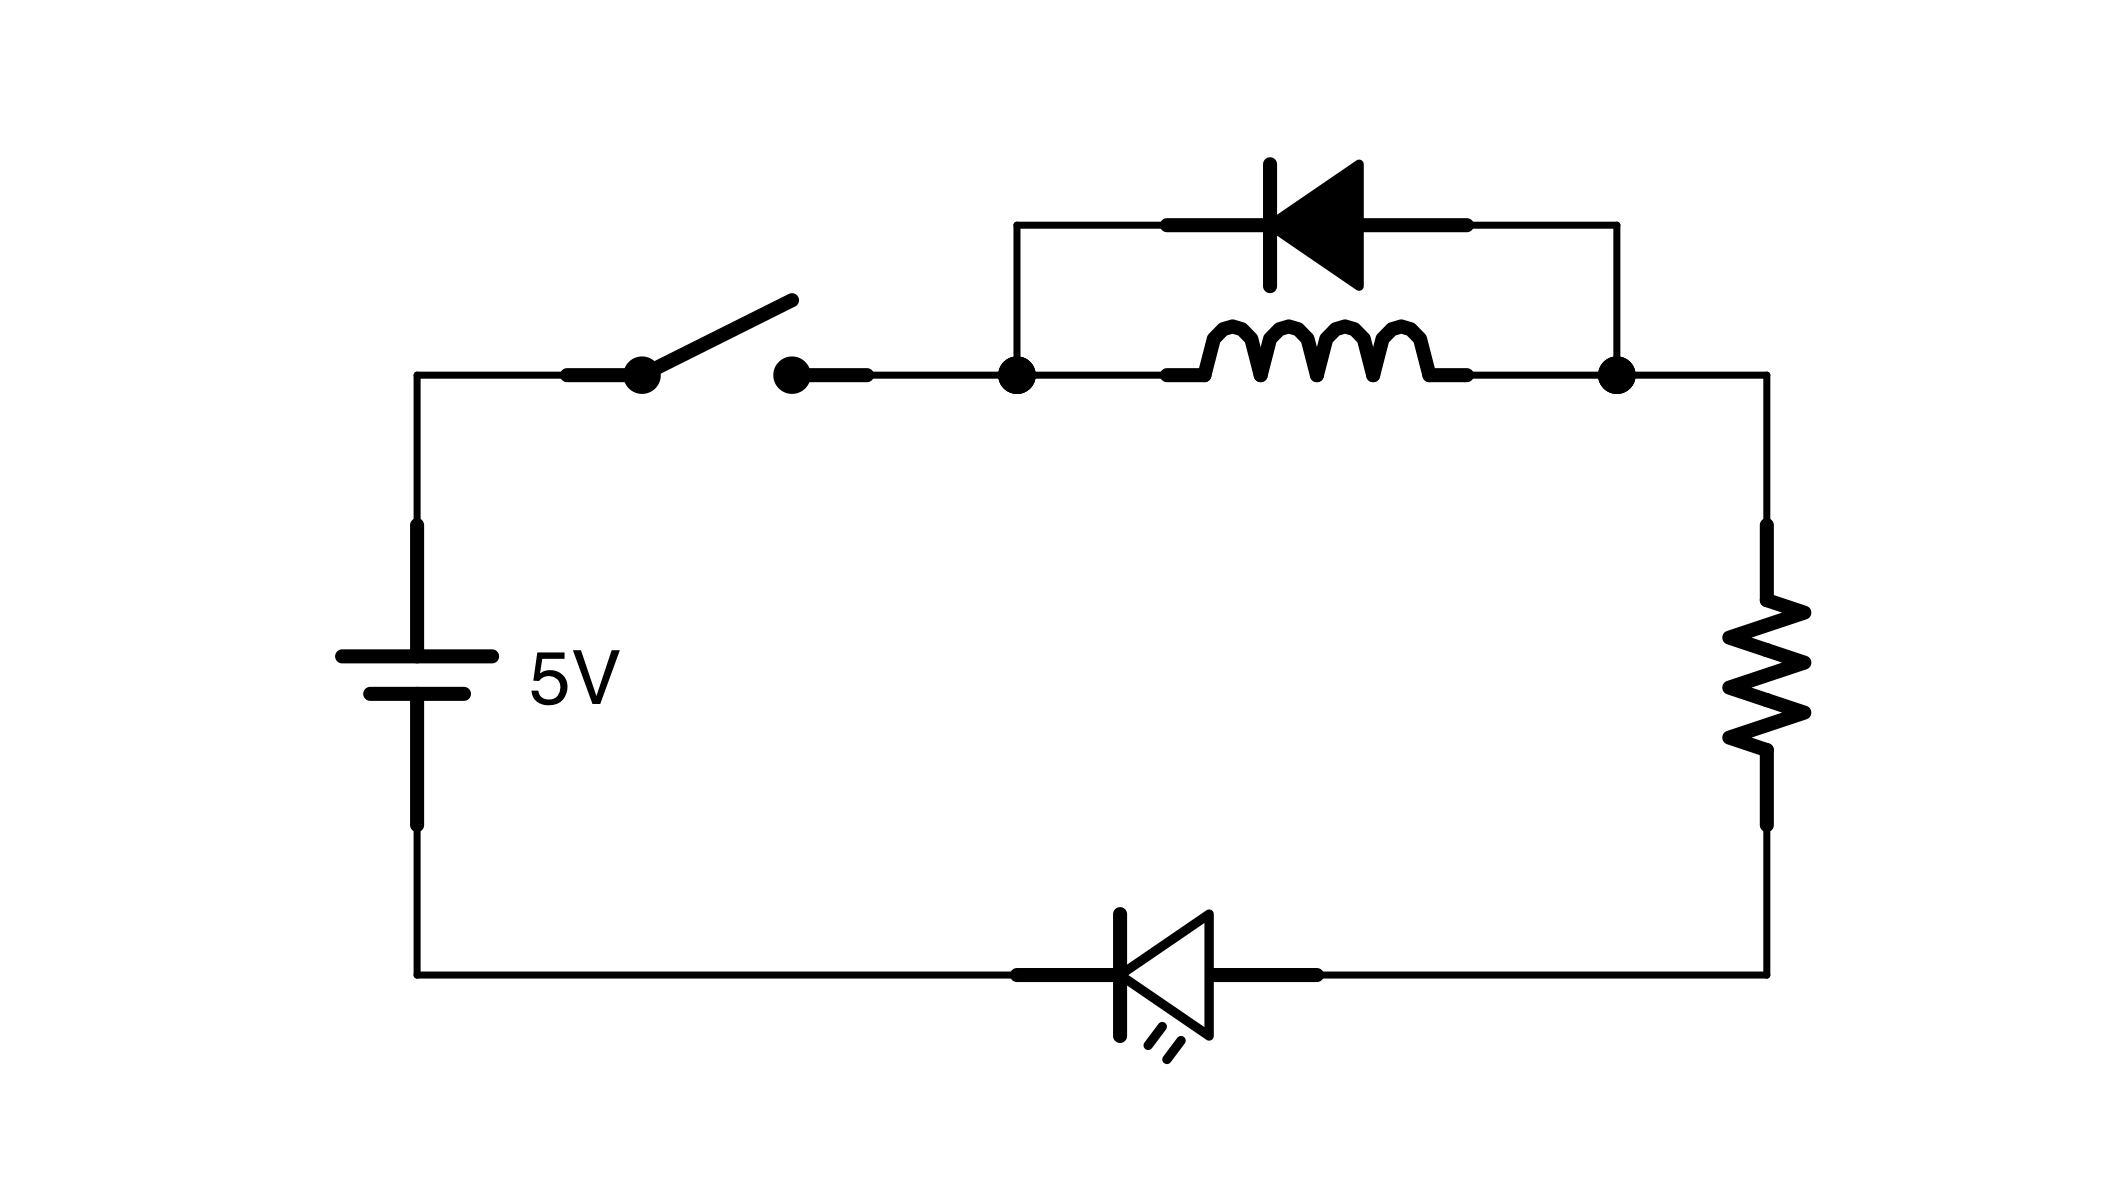
\includegraphics[width=0.7\columnwidth]{SolutionSnubberDiode.png}}
\item
\question{What is the purpose of the snubber diode?}
\solution{The snubber diode reduces the effect of the inductive kick by giving the current a pathway back through the inductor.
This allows generated voltages/currents to be bled off slowly throught the inductor itself.}
\item 
\question{If I have an inductor that is $5\myhy$ and has a steady current going through it of $2\myamp$, what is the size of the magnetic flux in the inductor's magnetic field?}
\solution{$10$ webers}
\explanation{The equation governing the behavior of an inductor is given by Equation~\ref{eqinductance}, $\phi = L \cdot I$, where $L$ is given in henries and $I$ is in amperes.
Therefore, since the units match, we can calculate as follows:
\begin{align*}
\phi &= L \cdot I \\
 &= 5 \cdot 2 \\
 &= 10
\end{align*}
Therefore, the inductor is holding $10$ webers of flux.
}
\item 
\question{If I have an inductor that is $7\myuhy$ and has a steady current going through it of $3\mymamp$, what is the size of the magnetic flux in the inductor's magnetic field?}
\solution{$0.000000021$ webers}
\explanation{The equation for flux is $\phi = L \cdot I$, where $L$  is in henries and $I$ is in amperes.
Therefore, we need to convert into proper units to use the equation.
Since $1\myuhy = 0.000001\myhy$, $7\myuhy = 0.000007\myhy$.
Since $1\mymamp = 0.001\myamp$, $3\mymamp = 0.003\myamp$.
Therefore, the equation becomes:
\begin{align*}
\phi &= L \cdot I \\
 &= 0.000007 \cdot 0.03 \\
 &=0.000000021
\end{align*}
Therefore, the magnetic field has a flux of $0.000000021$ webers.
}
\item 
\question{If I have a $4\myhy$ inductor with $0.3\mywb$ of flux in its magnetic field, how much current is flowing through it?}
\solution{$0.075\myamp$ or $75\mymamp$}
\explanation{We will solve this problem by rearranging Equation~\ref{eqinductance} to solve for $I$:
\begin{align*}
\phi &= L \cdot I \\
I &= \frac{\phi}{L}
\end{align*}
Since the units are already correct, I can now just substitute and solve:
\begin{align*}
I &= \frac{\phi}{L} \\
 &= \frac{0.3}{4} \\
 &= 0.075
\end{align*}
Therefore, the current is $0.075\myamp$ or $75\mymamp$.
}
\item 
\question{If an inductor's magnetic field has $5\mywb$ of flux and it decreases to $3\mywb$ of flux over $2\mysec$, what is the average voltage produced over that timeframe?}
\solution{}
\explanation{Questions involving the \emph{change} of voltage and flux utilize Equation~\ref{eqlenz}, which states:
\begin{align*}
V_{average} = -\frac{\textrm{change in }\phi}{\textrm{change in time}}
\end{align*}
Since we start with $5\mywb$ of flux and end with $3\mywb$, therefore, we changed by $-2\mywb$.
Since this occurred across $2\mysec$, the resulting formula would be:
\begin{align*}
V_{average} &= -\frac{-2}{2} \\
  &= 1
\end{align*}
Therefore, the average voltage produced for that time period is $1\myvolt$.
}
\item 
\question{If an inductor's magnetic field has $1\myuwb$ of flux and it increases to $2\myuwb$ of flux over $0.4\mysec$, what is the average voltage produced over that timeframe?}
\solution{}
\explanation{Questions involving the \emph{change} of voltage and flux utilize Equation~\ref{eqlenz}.  To use this equation, first we have to convert units.
The standard conversion is $1\myuwb = 0.000001\mywb$.
Therefore, the equation becomes:
\begin{align*}
V_{average} &= -\frac{\textrm{change in }\phi}{\textrm{change in time}} \\
 &= -\frac{0.000001}{0.4} \\
 &= -0.0000025
\end{align*}
Therefore, the inductor will produce a negative voltage, averaging $-0.0000025\myvolt$ for the duration of the $0.4\mysec$.
}
\item 
\question{If the current flowing through a $3\myhy$ inductor drops from $7\mymamp$ to $1\mymamp$ over a period of $0.01\mysec$, what is the average voltage produced over that time period?}
\solution{$1.8\myvolt$}
\explanation{To solve this, you will need \emph{both} Equation~\ref{eqinductance} and Equation~\ref{eqlenz}.
Equation~\ref{eqlenz} requires a starting and an ending flux. 
However, we are not given the starting and ending flux, but rather the starting and ending current.
Equation~\ref{eqinductance} tells us how to relate current to the amount of flux.

First, we need to convert our units.
$7\mymamp = 0.007\myamp$ and $1\mymamp = 0.001\myamp$.
Let's begin by solving for the starting flux:
\begin{align*}
\phi &= L \cdot I \\
 &= 3 \cdot 0.007 \\
 &= 0.021
\end{align*}
So the starting flux is $0.021\mywb$.

Next, let's solve for the final flux:
\begin{align*}
\phi &= L \cdot I \\
 &= 3 \cdot 0.001 \\
 &= 0.003
\end{align*}
So, the final flux is $0.003\mywb$.
This means that the change in flux was $-0.018\mywb$ across $0.01\mysec$.
Therefore, the average voltage over that period can be found using Equation~\ref{eqlenz}:
\begin{align*}
V_{average} &= -\frac{\textrm{change in }\phi}{\textrm{change in time}} \\
 &= -\frac{-0.018}{0.01} \\
 &= 1.8
\end{align*}
Therefore, the average voltage produced by the decrease in current over that time period is $1.8\myvolt$.
}
\end{enumerate}
